Таким образом, решено было использовать эвристические алгоритмы оптимизации:
\href{https://en.wikipedia.org/wiki/Simulated_annealing}{Генетический алгоритм} и \href{https://en.wikipedia.org/wiki/Simulated_annealing}{Симуляция отжига}.
Подробное описание алгоритмов, моей их реализации и улучшений представлено в секции \ref{sec:opimization_algorithms}.

\subsection{Представление «решения»  — набора мазков}
Программа работает с последовательностями мазков, находя лучшую из них.
Однако, чтобы алгоритм оптимизации работал с ними, наборы мазков должны быть представлены в виде векторов в $\mathbb{R}^n$.
Формат данных в «геноме» таков:

\begin{figure}[h]
    \centering
    \adjincludegraphics[width=0.7\textwidth, clip, trim={0.15\width} {0.7\height} {0.15\width} {0.125\height}]{genome_contents_table.pdf}
    \caption{Схема хранения генома}
    \label{fig:genome_contents_table}
\end{figure}


, где $p_{n_x} ~\&\&~ p_{n_y}, n \in \{ 0, 1, 2 \}$ — координаты направляющей точки под номером n (из всего 3 у каждого мазка),
а \textit{width}  — толщина мазка.

Здесь нет параметра  «цвет».
Причина объяснена в разделе: \ref{subsec:color_in_genome}.

\subsection{Задание функции ошибки}
Чтобы решить задачу алгоритмом оптимизации, нужна некая метрика — функция, которая будет определять степень «неподходящести» данного ей решения.
Именно она будет передаваться алгоритму оптимизации.
В нашем случае вычисление функции ошибки (далее — ФО) включает в себя растеризацию мазков (отображение их на изображении) и вычисления, производящие сравнения полученного результата с желаемым.
ФО необходимо задать таким образом, чтобы она отражала качество полученной комбинации мазков,
причём в любой точке направление её уменьшения соответствовало направлению улучшения результата.
За основу была выбрана \href{https://en.wikipedia.org/wiki/Mean_squared_error}{MSE} (Mean Square Error):

\begin{equation}\label{eq:equation}
    MSE = \frac{1}{width \cdot height} \cdot \sum_{y = 0}^{y < height} { \sum_{x = 0}^{x < width} { \sum_{c \in  \left\{ r, g, b \right\} } { \left( {\overrightarrow {rendered_{x, y}}}_c - {\overrightarrow{original_{x, y}}}_c\right)^2 }}}
\end{equation}

MSE — универасльная мертрика для схожести изображений, она повсеместно используется при работе с ними.
Но в нашем случае, о чём свидетельствует практика, целесообразно добавить в ФО компоненту, «наказывающую» за наложение мазков друг на друга, а также за пустые (ничем не закрашенные) места.

Первое улучшение очевидно — при прочих равных лучше ситуация, при которой та же картина достигнута с меньшим использованием краски
(а если не вводить эту компоненту, наложено в найденном решении может быть сразу много (> 2) мазков в одной точке).
Если нет разницы, зачем переплачивать?

С теоретической точки зрения может быть непонятна надбавка за пустоты: ведь если место пустое, оно и так не даёт оптимальное MSE.
Однако на практике пусто́ты недостаточно быстро и полно покрываются (особенно — на ускоренном режиме) без этой надбавки.

Таким образом, функция ошибки сделана так, чтобы максимально стимулировать правильно распределение мазков.

\subsection{Растеризация мазков}\label{subsec:rasterization}
Имея мазок, заданный в виде трёх точек на плоскости, толщины и цвета, нужно уметь его отобразить его на «холсте», то есть в виде набора пикселей.
Это нужно, чтобы подсчитать функцию ошибки для заданного набора мазков,
причём так, чтобы результат максимально соответствовал мазку, рисуемому роботом.
В качестве достаточно точной модели описания такого мазка возьмём круглую кисть, перемещающуюся по заданной траектории.
Есть много способов произвести растеризацию.
Нужно выбрать тот, который будет производительным и в то же время максимально близким к реальному мазку.

Самый простой — для некоторого количества точек на кривой Безье (с достаточно маленьким шагом, примерно один пиксель) проводим вертикальную линию: вверх на width и  вниз — тоже.
Это даёт высокую производительность и сносно выглядит на участках, близких к горизонтальным, но результат, полученный таким способом, очень далёк от реальности на вертикальных участках:
\begin{figure}[h!]
    \centering
    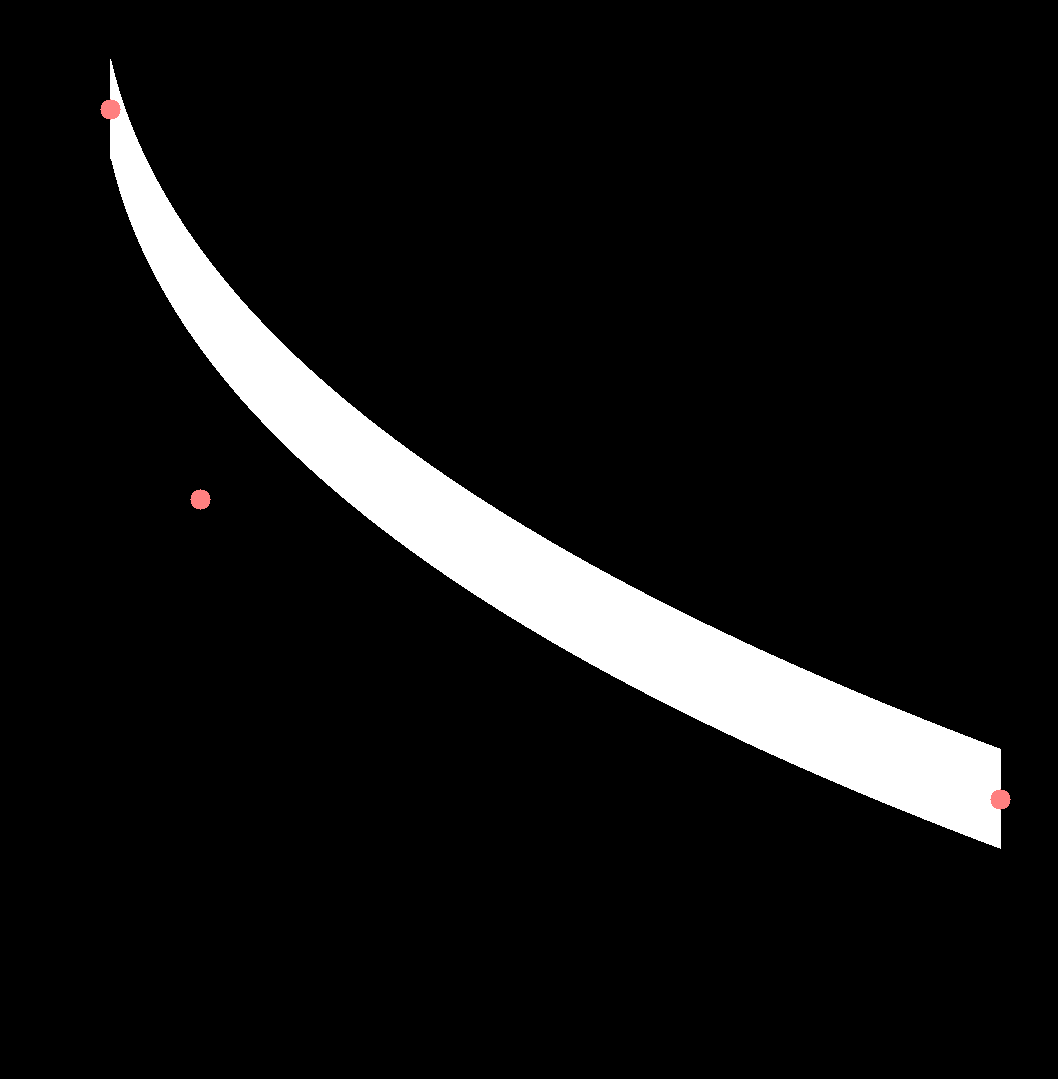
\includegraphics[width=0.75\textwidth]{stroke_vertical.png}
    \caption{(Красным обозначены точки, задающие кривую)}
    \label{fig:vertical_stroke}
\end{figure}
\begin{figure}
    \centering
    
\includegraphics[width=0.75\textwidth]{one_stroke.png}
    \caption{Иногда такой способ добавляет свой шарм}
    \label{fig:pretty_vert_stroke}
\end{figure}

Есть разные способы избавиться от этих недостатков, сохраняя максимальную производительность.
Например:
\begin{itemize}
    \item Совмещать горизонтальные и вертикальные полосы
    \item Проводить полосы перпендикулярно направлению кривой в данной точке
\end{itemize}
В каждом из них будут наблюдаться пустые места, полости, что недопустимо.

Ультимативным же способом является подражание реальной жизни: «проведение» круглой «кистью» по экрану.
То есть берутся точки на кривой на небольшом расстоянии друг от друга, далее из каждой рисуется круг радиусом width.
Однако в таком случае каждая точка, попадающая в мазок, обрабатывается много раз (для близких кругов), что значительно замедляет рендерниг.
Если же увеличить шаг, этой проблемы можно частично избежать, но мазок стал бы неровным.
При маленьком шаге это выглядит так:
\begin{figure}[h!]
    \centering
    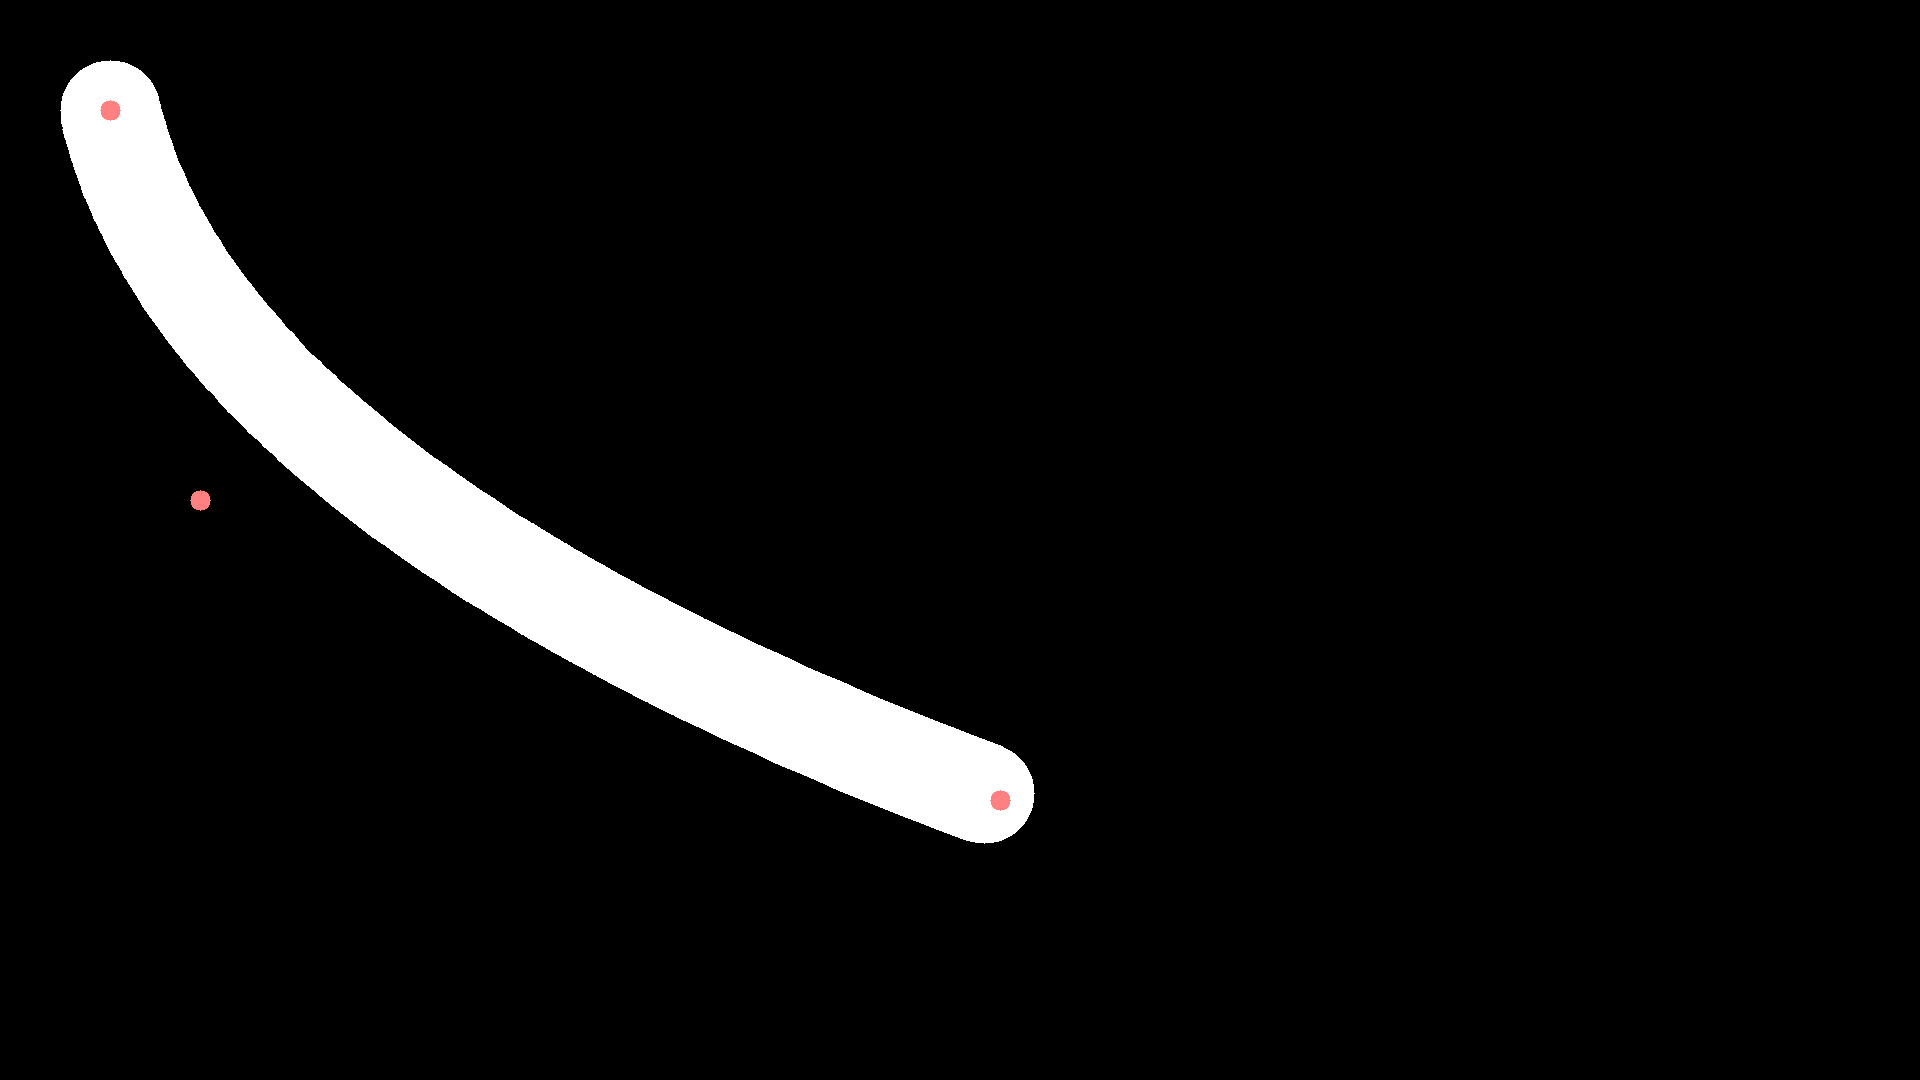
\includegraphics[width=0.75\textwidth]{stroke_smooth.png}
    \label{fig:smooth_stroke}
\end{figure}

В будущем планируется улучшить алгоритм для ускорения растеризации при почти том же качестве.
Рассматриваются варианты:
\begin{itemize}
    \item Заменить круглую кисть на также гладкую, но с более медленным закруглением с дальней от вектора кривой в данной точке стороны, поворачивая кисть соответствующим образом:
    \begin{figure}[h!]
        \centering
        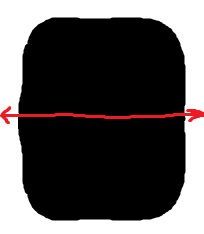
\includegraphics[width=0.75\textwidth]{modern_brush.png}
        \caption{(красным обозначено направление вектора кривой)}
        \label{fig:modern_brush}
    \end{figure}
    Такое изменение поможет уменьшить артефакты при увеличении шага между точками на кривой, то есть позволит сделать шаг больше, ускорив процесс.

    \item Автоматически разбивать мазок на «полигоны».
                Для этого нужно пройтись по кривой и с некоторым шагом (уже побольше, чем раньше),
                отметить для каждой рассматриваемой точки на прямой, содержащей её и перпендикулярной текущему направлению, точки в обе стороны от неё на расстоянии width.
                Каждая из них добавляется в соответствующий стороне в порядке обхода список.
                Потом полигоны, полученные из соседних точек на кривой и соответствующим им вынесенным точкам, заливаются нужным цветом.
                На концах же мазка рендерятся круги.

    \begin{figure}[h!]
        \centering
        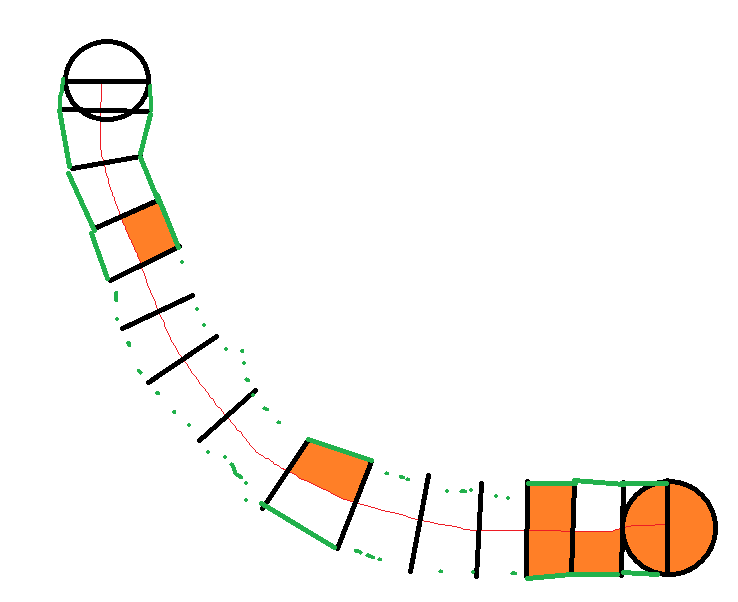
\includegraphics[width=0.75\textwidth]{polygonal_stroke.png}
        \caption{Схема полигональной разбивки мазка}
        \label{fig:polygonal_stroke}
    \end{figure}

    При использовании этого метода никакая существенная часть пикселей мазка не обрабатывается много раз, что говорит о высокой эффективности алгоритма.
    Поэтому я собираюсь внедрить такой метод в ближайшее время.
\end{itemize}

Что же касается совместимости с видеокартой,
для круга и модифицированной кисти понятно, как определить bouding-box,
и понятно, как по координатам пикселя быстро определить, принадлежит ли он этому примитиву.
А рендеринг полигонов производится аппаратно.

Подробнее про внедрение видеокарты можно почитать в разделе \ref{subsec:move_graphics_to_videocard}.


\subsection{Учёт цвета при оптимизации}\label{subsec:color_in_genome}

\subsubsection{Знание цвета при рендеринге необходимо}
Цвет является обязательным параметром мазка, без которого непонятно, как его растеризовать.
Но значит ли это, что цвет обязательно должен быть одним из параметров алгоритма оптимизации?
Конечно же, нет.

\subsubsection{Определение цвета по положению при подсчёте ФО}
Во-первых, цвет может быть легко определён, зная положение.
Самый простой способ — найти среднее арифметическое цветов пикселей.
Мы автоматически получим минимальное MSE,
так как для каждой из цветовых компонент соответствующая часть MSE — сумма квадратичных функций (для каждого пикселя),
причём «с ветвями вверх» (так как на бесконечностях она уходит в $+ \infty$), которая имеет одну точку с нулевой производной — как раз в среднем арифметическом:

\begin{equation}
    \begin{gathered}
        MSE_c(value_c) = \sum_{pixel \in {pixels}} \bigg(value_c - pixel_c\bigg)^2 \\
        \Rightarrow \\
        MSE_c'(value_c) = 2 \cdot \left( \lVert pixels \lVert \cdot value_c - \sum_{pixel \in {pixels}}  pixel_c \right)
    \end{gathered}
\end{equation}
, где $pixel_c$ — значение канала $c$ пикселя $pixel$.

То есть у MSE достигается производная ноль в этой точке:
\begin{equation}
    MSE_c'(value_c) = 0
    \Longleftrightarrow
    value_c = \frac{\sum_{pixel \in {pixels}}  pixel_c}{\lVert pixels \lVert} = \overline{pixel}
\end{equation}
Следовательно, больше нигде ноль не достигается, так как функция квадратичная.
Более того, это минимум, так как функция — «ветви кверху».

\subsubsection{Фиксированный цвет в зонах}
Во-вторых, при делении на зоны все пиксели, относящиеся к данной зоне, имеют строго заданный цвет.
Подробнее об этом читать в секции \ref{subsec:applying_zoning}.


\subsection{Разделение картины на зоны}\label{subsec:applying_zoning}

\subsubsection{Обоснование эффективности}\label{subsubsec:why_split_into_zones}
Известно, что время оптимизации до заданного качества очень сильно увеличивается при увеличении количества параметров.
Причём существенно более быстро, чем линейно.
Следовательно, можно получить выгоду, разделяя эти параметры каким-то образом и оптимизируя группы по отдельности.
\begin{equation}
    F(\lVert parameters \lVert) \ggg n \times F  \left( \frac{\lVert parameters \lVert}{n} \right)
\end{equation}

Вопрос в том, в каких случаях это делать можно (то есть в каких случаях качество оптимизации заметно не уменьшится при разбиении), а в каких — нет.

Надо понимать, что нельзя независимо оптимизировать близкие мазки: только их комбинация позволит понять,
хорошо ли предпринятое изменение для каждого и для всех в целом.
Находить положение одного, не зная положение другого, почти бесполезно.
Однако, если мазки находятся далеко друг от друга, можно безболезненно произвести деление.

\textcolor{gray}{Пояснение: Применительно к данной задаче супераддитивность времени выполнения алгоритма по отношению к размерности входного пространства для функций в целом
можно описать так: если мутация затрагивает большое количество мазков из разных сторон изображения, «картина» для функции ошибки очень зашумлена:
если ФО увеличилась, определить, следствием какой именно части мутаций было то или иное изменение ФО, можно только очень «некачественно» (то есть с малой вероятностью).
А следовательно, мутации будут хаотично приниматься и наслаиваться, но это не обеспечит устойчивого движение к оптимуму через комбинирование правильных мутаций.
Причём выбор маленького количества трансформаций за мутацию — не выход: нужно именно не такое малое количество изменений за один раз, причём таких, чтобы они были рядом,
то есть сильно влияли друг на друга.
А совсем малое количество изменений за мутацию — плохо, так как эти переменные сильно зависимы друг от друга, оптимизация, например, сначала по одной, потом по другой и т.д.
приведёт не к нахождению глобального оптимума, а к застреванию в локальном.
Чтобы выйти из него, нужно изменение сразу большого количества переменных.
Конечно, ГА — это не \textit{Hill climbing algorithm}, он не «отрезает» сразу любое изменение, не приведшее к результату,
но вышеупомянутые механизмы всё равно привозят к уменьшению производительности при слишком маленьком количестве изменений за одну мутацию.}

Поэтому (так как важно немалое количество изменений, сконцентрированных в одном месте, чтобы избежать попадания в локальный оптимум, — с одной стороны
и отсутствие сбивания \sout{рыночных} целевофункциевых сигналов другими частями картины),
важно как-либо разделять изображения на зоны:
функция ошибки сепарабельна, но только до какого-то размера зоны, при малом количестве мазков, близких друг другу, это перестаёт работать.


\subsubsection{Прямоугольные зоны}
Проще всего в реализации — делить изображение на прямоугольные зоны.
Каждая рассматривается как отдельное изображение, для него находятся мазки, которые потом со сдвигом добавляются «в общий котёл».

Встаёт очевидный вопрос: как избежать заметности границ этих зон на финальном изображении?

Первое средство — расчерчивать эти границы наложенными друг на друга.
То, какую часть перекрытие должно составлять от всей зоны, можно настроить эмпирически, запуская программу с разными значениями этого параметра
и сравнивая плотность в местах стыка и на остальной картине.
Подобранное значение почти универсально, то есть может быть применено и для обработки других картин.

Второе средство — после получения результатов для зон «разблокировать положение» мазков, лежащих рядом со стыками,
запустив оптимизацию для них уже на основе данных целой картины.
Конечно, и здесь имеет смысл отдельно оптимизировать «кресты», образующиеся при стыке четырёх зон.
Также можно в качестве ограничений использовать не весь box картины, а зоны этих крестов.
Более того, если окажется, что плотности в местах стыка будет не хватать, можно добавить некоторое количество новых мазков (т.н. клеящего вещества).

Последние улучшения не были внедрены, так как $\downarrow\downarrow\downarrow$ % \symbol{"21A1}\symbol{"21A1}\symbol{"21A1} % ↡↡↡

\subsubsection{Зоны произвольной формы}
Понятно, что лучшее качество даёт деление на зоны, связанное со структурой картинки.
То есть цвет должен несильно меняться в пределах зоны.
Вопрос в том, как изображение на такие зоны поделить.

Такие программы, как Adobe Illustrator, умеют эту выполнять эту операцию (правда, с некоторыми проблемами, о них — позже).



% TODO: переместить описание проблем и их решений сюда…


\subsection{Сортировка мазков перед выпуском}\label{subsec:stroke_sorting}

В случае растеризации набора мазков на компьютере время выполнения операции почти совсем не зависит от порядка следования мазков
(если не считать незаметное влияние кэширования в процессоре), так как закрашивание пикселя происходит через \textit{random access}.
Однако в реальности это далеко не так: правильный порядок мазков (как по координатам, так и по цветам) может сильно уменьшить время отрисовки, которое весьма велико,
и поэтому нельзя забывать про задачу правильного расположения мазков.

\subsubsection{Сортировка по территориальному признаку}
В первом приближении количество цветов очень небольшое (скорее всего, не больше десяти),
а, чтобы сменить цвет, нужно вести кисть к банке с водой, смывать краску предыдущего цвета, брать новый,
а потом опять несть кисть через весь стол.
Поэтому разумно сначала разделить мазки на группы по цветам, а в каждой из них располагать их так,
чтобы минимизировать пройденное кистью расстояние при последовательной отрисовке мазков этого цвета.

% TODO: задача Комивояжёра!!!

Конечно, можно оформить нахождение лучшей последовательности как оптимизационную задачу,
но это будет неоправданно ресурсозатратно, так как от задачи зависит только скорость рисование, но не качество конечного продукта.

Достаточное качество даёт … (зоны, внутри них), но рассматривается использование \href{https://en.wikipedia.org/wiki/Christofides_algorithm}{алгоритма Кристофидеса}.

\subsubsection{Оптимальная расстановка цветов}

